% Appendix C

\chapter{Work Breakdown Structure} % Main appendix title

\label{AppendixC} % For referencing this appendix elsewhere, use \ref{AppendixC}

O âmbito deste projeto foi decomposto através de um \gls{WBS}. Pelo mesmo, ilustrado na Figura \ref{fig:wbs}, estão organizados os entregáveis previstos por cinco fases principais, sendo estas:

\begin{enumerate}
    \item \textbf{Planeamento e Análise:} Focada na definição do problema e estado da arte. Inclui entregáveis como o Project Charter, o próprio \gls{WBS}, um Gantt Chart, um questionário e respetivas respostas dos \glspl{OPC}, este Extended Abstract e a revisão da literatura incluída no mesmo.
    \item \textbf{Design:} Dedicada à modelação da solução. Os principais entregáveis previstos são a documentação da Arquitetura de Software (Vistas 4+1) e o Modelo de Domínio, assegurando que a estrutura do \gls{FUSE} é robusta antes da implementação.
    \item \textbf{Desenvolvimento:} Fase central do projeto, onde será implementado o código da aplicação. Divide-se em três módulos críticos: Comunicações Seguras, Camada de Abstração e Módulo de Análise de Vídeo.
    \item \textbf{Testes:} Validação da solução através de testes unitários e funcionais, em conjunto com a validação do protótipo em ambiente controlado ou cenário real.
    \item \textbf{Conclusões:} Considerações finais do projeto, incluindo a redação final da dissertação, a interpretação dos resultados e a apresentação final.
\end{enumerate}

\begin{figure}[H]
\centering
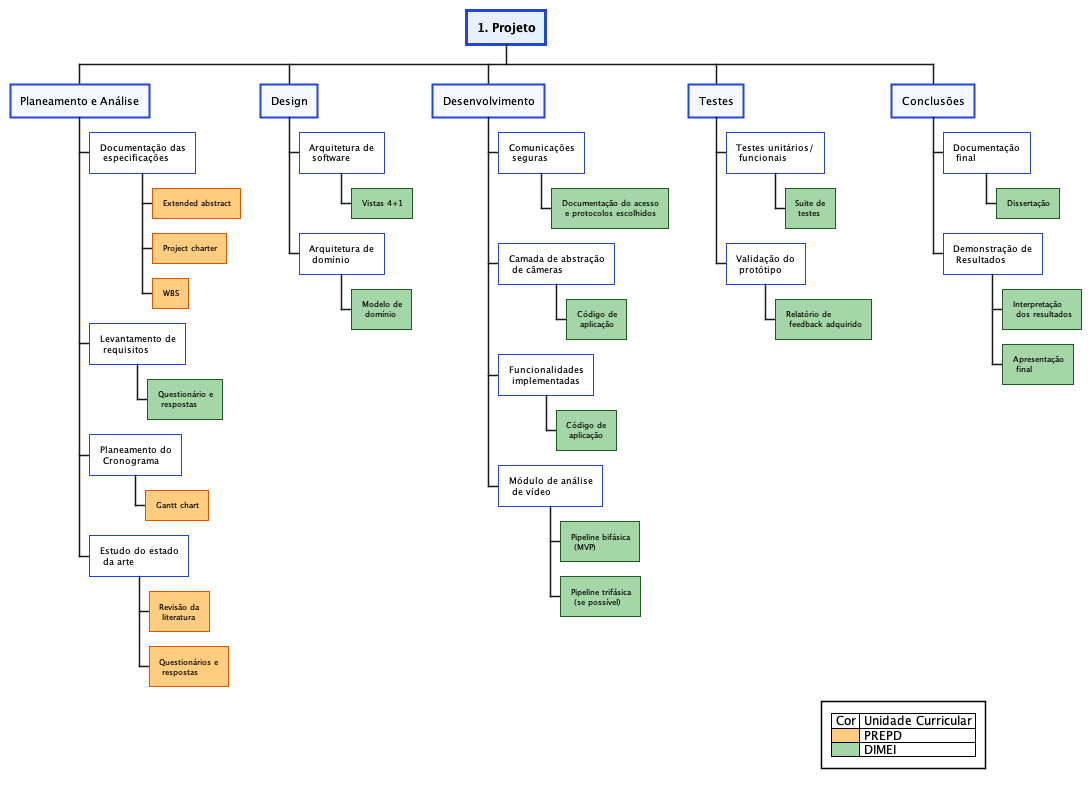
\includegraphics[width=\textwidth]{appendices/assets/WBS.png}
\caption{WBS do projeto.}
\label{fig:wbs}
\end{figure}
